%!Tex Root=**/main.tex
\mode<presentation>{\subsection{Feature-3DGS}}
\mode<article>{\section{Feature-3DGS}}
\begin{frame}
	\Frametitle{Overview}
	\mode<presentation>{\blfootnote{\href{http://arxiv.org/abs/2312.03203}{(CVPR Highlight, 2024) Feature 3DGS: Supercharging 3D Gaussian Splatting to Enable Distilled Feature Fields}}}
	\mode<article>{Figure~\ref{fig:feature-3DGS-overview} is the tagged framework figure of Feature 3DGS~\autocite{zhouFeature3DGSSupercharging2024apr}.}
	\begin{figure}[htbp]
		\begin{annotatedFigureEnv}
			{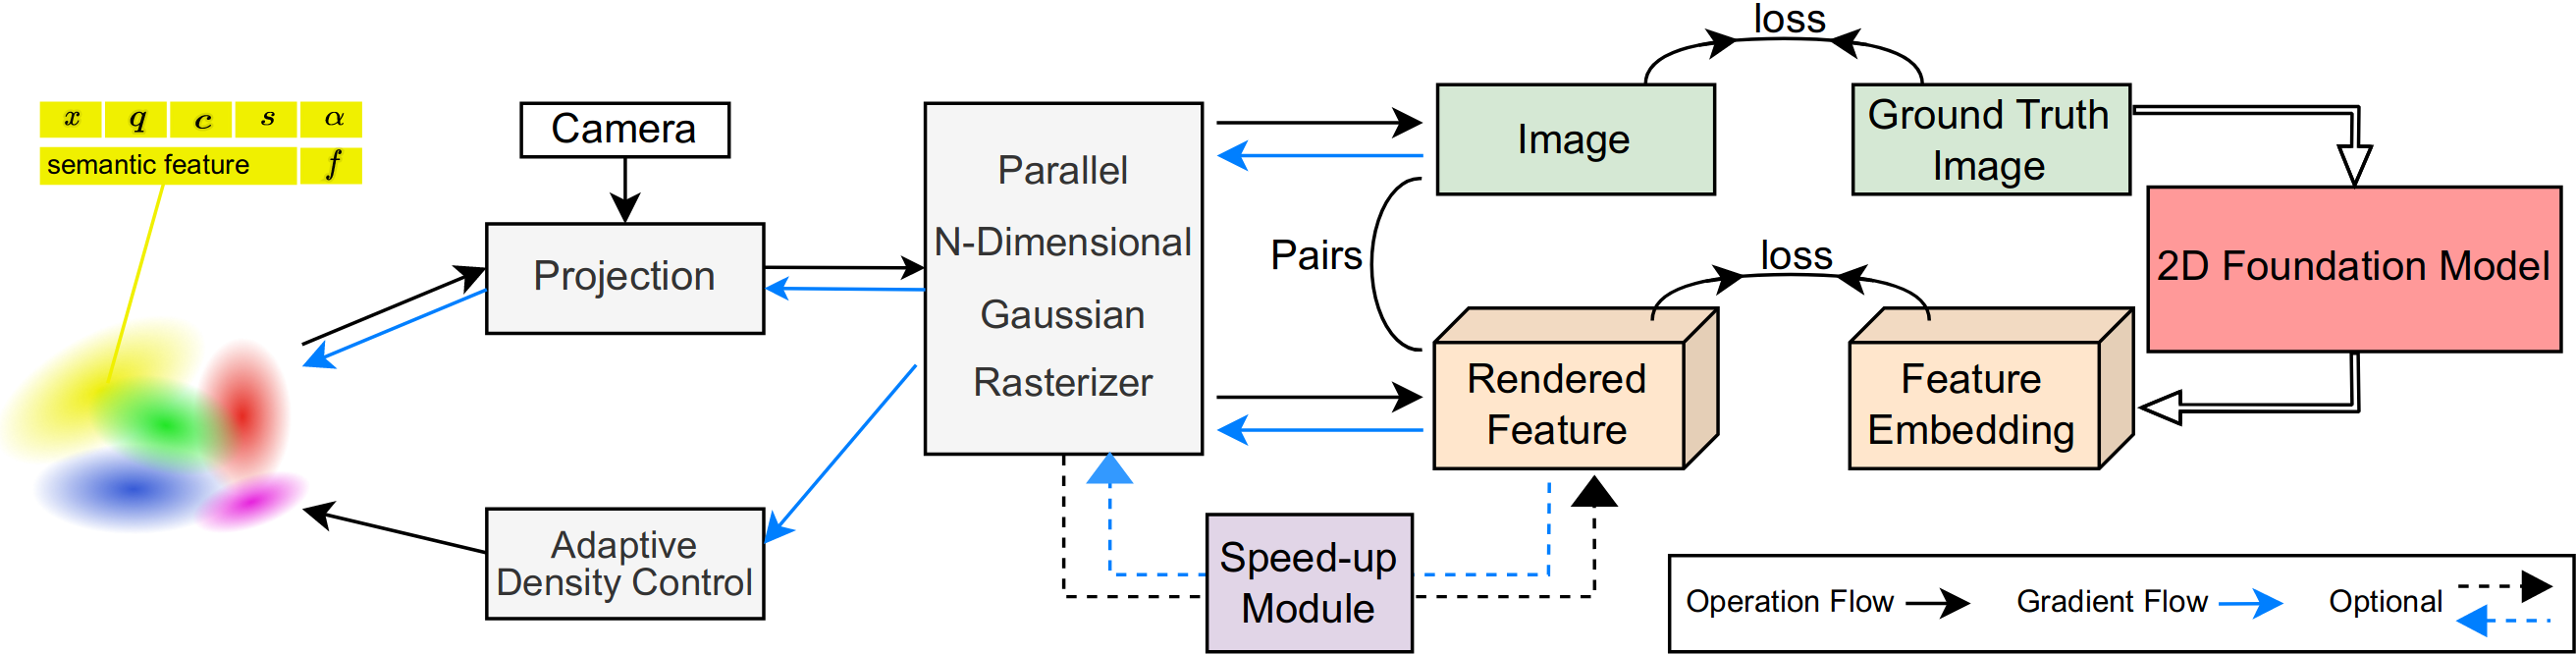
\includegraphics[width=0.85\linewidth]{feature-3dgs-overview.png}}
			\only<1|handout:1>{\annotatedFigure{0,0.7}{0.15,0.78}{1}{0,0.74}}
			\only<1|handout:1>{\annotatedFigure{0.55,0.25}{1,0.72}{1}{0.55,0.72}}
			\only<2->{\annotatedFigure{0.45,-0.05}{0.57,0.25}{2}{0.45,0.25}}
		\end{annotatedFigureEnv}
		\vspace*{0.5ex}
        \caption{Overview of Feature 3DGS~\autocite{zhouFeature3DGSSupercharging2024apr}}
		\label{fig:feature-3DGS-overview}
	\end{figure}
	\mode<presentation>{\vspace*{\fill}}
	\begin{block}{Key Insights}
		\begin{enumerate}
			\mode<presentation>{\setlength{\itemsep}{1.5ex}}
			\item<1-> \alert<1>{Semantic Rendering Pipeline}
				\mode<presentation>{\vspace*{1.5ex}}
				\par Differentiable rendering of Gaussian-wise latent semantic features.
			\item<2-> \alert<2>{Speed-up module}
				\mode<presentation>{\vspace*{1.5ex}}
				\par Dimensionality Alignment.
		\end{enumerate}
	\end{block}
\end{frame}

\begin{frame}\Frametitle{Semantic Rendering Pipeline}
	\mode<presentation>{\blfootnote{\href{http://arxiv.org/abs/2312.03203}{(CVPR Highlight, 2024) Feature 3DGS: Supercharging 3D Gaussian Splatting to Enable Distilled Feature Fields}}}
	\par To render semantic embeddings, i.e. \mode<article>{equation~\ref{eq:feature-3dgs-semantic-rendering}, we have 5 notable things.}
	\begin{figure}[htbp]
		\centering
		\vspace*{2em}
		\resetcolorseries[4]{marknode-color-series}
		\resetcolorseries[4]{annotation-color-series}
		\begin{equation}\label{eq:feature-3dgs-semantic-rendering}
			\mathbb{R}^{
			\alt<3->{\tikzmarknode{n1}{\colorbox{marknode-color-series!![1]}{\scriptsize \(D\)}}}{D}
			}
			\times
			\left\{0,1,\cdots,
			\alt<2->{\tikzmarknode{n0}{\colorbox{marknode-color-series!![0]}{\(N\)}}}{N}
			\right\}
			\times
			\alt<4->{\tikzmarknode{n2}{\colorbox{marknode-color-series!![2]}{\(\left\{\mathcal{F}\right\}\)}}}{\left\{\mathcal{F}\right\}}
			\mapsto
			\left\{0,1,\cdots,
			\alt<5->{\tikzmarknode{n3}{\colorbox{marknode-color-series!![3]}{\(H\)}}}{H}
			\right\}
			\times
			\left\{0,1,\cdots,
			\alt<6->{\tikzmarknode{n4}{\colorbox{marknode-color-series!![4]}{\(W\)}}}{W}
			\right\}
			\times
			\mathbb{R}^{D}
		\end{equation}
		\begin{annotatedEquationEnv}
			\only<2->{\annotatedEquation{colorseries}{n0}{north}{0em}{0.5em}{south west}{annotation-color-series}{number of 3D Gaussians}{east}}
			\only<3->{\annotatedEquation{colorseries}{n1}{north}{0em}{2em}{south west}{annotation-color-series}{dimension of semantic embedding}{east}}
			\only<4->{\annotatedEquation{colorseries}{n2}{south}{0em}{-0.5em}{north east}{annotation-color-series}{camera frames}{west}}
			\only<5->{\annotatedEquation{colorseries}{n3}{south}{0em}{-0.5em}{north east}{annotation-color-series}{image height}{west}}
			\only<6->{\annotatedEquation{colorseries}{n4}{south}{0em}{-0.5em}{north east}{annotation-color-series}{image width}{west}}
		\end{annotatedEquationEnv}
		\vspace*{0.5em}
	\end{figure}
	\mode<presentation>{
		\mode<presentation>{\vspace*{\fill}}
		\begin{minipage}[c]{0.35\linewidth}
			\definecolor{feature-3dgs-blue}{HTML}{007FFF}
			\uncover<7->{\par 5 things,}
			\mode<presentation>{\vspace*{1.5ex}}
			\begin{enumerate}[<+(7)- |alert@.(8)>]
				\mode<presentation>{\setlength{\itemsep}{1.5ex}}
				\item representation
				\item projection
				\item blending
				\item rasterization
				\item \textcolor{feature-3dgs-blue}{inverse rendering}
			\end{enumerate}
		\end{minipage}
		\mode<presentation>{\begin{minipage}[c]{0.60\linewidth}
				\centering
				\begin{uncoverenv}<7->
					\adjustbox{trim={.01\width} {.01\height} {.5\width} {.1\height}, clip}{
						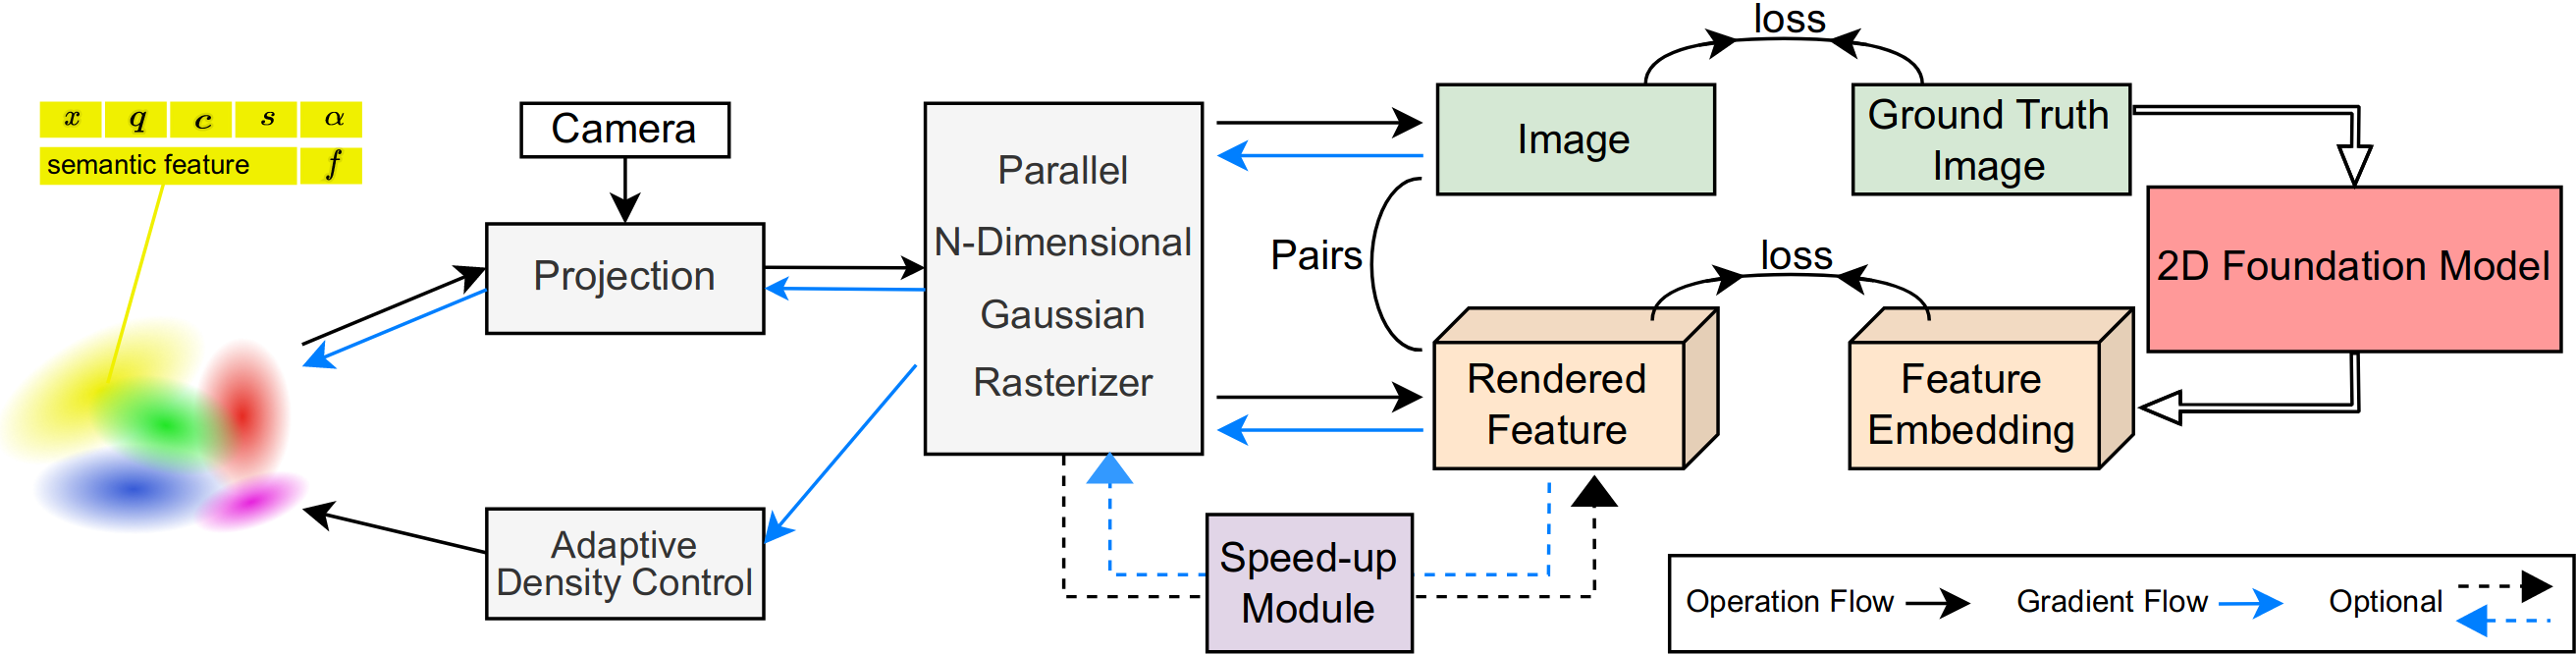
\includegraphics[width=1.5\linewidth]{feature-3dgs-overview.png}
					}
				\end{uncoverenv}
			\end{minipage}}
	}
\end{frame}

\begin{frame}\mode<presentation>{\Frametitle{Semantic Rendering Pipeline \romannum{1}}}
	\mode<presentation>{\blfootnote{\href{http://arxiv.org/abs/2312.03203}{(CVPR Highlight, 2024) Feature 3DGS: Supercharging 3D Gaussian Splatting to Enable Distilled Feature Fields}}}
	\begin{block}{Representation\hfill Semantic Rendering Pipeline \romannum{1}}
		\par \alert<+>{Representation}: 3D Gaussian augmented with a latent embedding.
        \footnote{For color representation, \(n\) is the maximal order of spherical harmonics for a color channel. \(n=4\) in practice.}
        \mode<article>{(equation~\ref{eq:feature-3dgs-semantic-gaussian})}
		\resetcolorseries[8]{marknode-color-series}
		\resetcolorseries[8]{annotation-color-series}
		\begin{equation}\label{eq:feature-3dgs-semantic-gaussian}
			\alt<2-|handout:1>{\tikzmarknode{n0}{\colorbox{marknode-color-series!![0]}{\(\mathcal{G}\)}}}{\mathcal{G}}
			_{
			\alt<3-|handout:1>{\tikzmarknode{n1}{\colorbox{marknode-color-series!![1]}{\scriptsize \(i\)}}}{i}
			}
			=
			\left\{
			\alt<4-|handout:1>{\tikzmarknode{n2}{\colorbox{marknode-color-series!![2]}{\(\mathbf{x}\)},}}{\mathbf{x},}
			\alt<5-|handout:1>{\tikzmarknode{n3}{\colorbox{marknode-color-series!![3]}{\(\mathbf{q}\)},}}{\mathbf{q},}
			\alt<6-|handout:1>{\tikzmarknode{n4}{\colorbox{marknode-color-series!![4]}{\(\mathbf{s}\)},}}{\mathbf{s},}
			\alt<7-|handout:1>{\tikzmarknode{n5}{\colorbox{marknode-color-series!![5]}{\(\alpha\)},}}{\alpha,}
			\alt<8-|handout:1>{\tikzmarknode{n6}{\colorbox{marknode-color-series!![6]}{\(\mathbf{c}\)},}}{\mathbf{c},}
			\alt<9-|handout:1>{\tikzmarknode{n7}{\colorbox{marknode-color-series!![7]}{\(\mathbf{f}\)},}}{\mathbf{f}}
			\right\}
		\end{equation}
		\begin{annotatedEquationEnv}
			\only<2-|handout:1>{\annotatedEquation{colorseries}{n0}{south}{0em}{-0.5em}{north east}{annotation-color-series}{optimizable 3D Gaussian}{west}}
			\only<3-|handout:1>{\annotatedEquation{colorseries}{n1}{south}{0em}{-2em}{north east}{annotation-color-series}{\(\in \mathbb{N}\), index of 3D Gaussian}{west}}
			\only<4-|handout:1>{\annotatedEquation{colorseries}{n2}{south}{0em}{-8em}{north west}{annotation-color-series}{\(\in \mathbb{R}^{3}\), position}{east}}
			\only<5-|handout:1>{\annotatedEquation{colorseries}{n3}{south}{0em}{-6.5em}{north west}{annotation-color-series}{\(\in \mathrm{SO}(3)\), rotation}{east}}
			\only<6-|handout:1>{\annotatedEquation{colorseries}{n4}{south}{0em}{-5em}{north west}{annotation-color-series}{\(\in \mathbb{R}^{3}\), scale}{east}}
			\only<7-|handout:1>{\annotatedEquation{colorseries}{n5}{south}{0em}{-3.5em}{north west}{annotation-color-series}{\(\in [0,1]\), opacity}{east}}
			\only<8-|handout:1>{\annotatedEquation{colorseries}{n6}{south}{0em}{-2em}{north west}{annotation-color-series}{\(\in \mathbb{R}^{3n}\), color}{east}}
			\only<9-|handout:1>{\annotatedEquation{colorseries}{n7}{south}{0em}{-0.5em}{north west}{annotation-color-series}{\(\boldmath \in \mathbb{R}^{3}\), semantic feature}{east}}
		\end{annotatedEquationEnv}
		\vspace*{8em}
	\end{block}
\end{frame}

\begin{frame}
	\mode<presentation>{\Frametitle{Semantic Rendering Pipeline \romannum{2}}}

	\mode<presentation>{\blfootnote{\href{http://arxiv.org/abs/2312.03203}{(CVPR Highlight, 2024) Feature 3DGS: Supercharging 3D Gaussian Splatting to Enable Distilled Feature Fields}}}

	\begin{block}{Projection\hfill Semantic Rendering Pipeline \romannum{2}}
		\par \alert<.>{Projection}: from 3D ellipsoids to 2D ellipses. \mode<article>{(equation~\ref{eq:feature-3dgs-projection-mean} and~\ref{eq:feature-3dgs-projection-covariance})}
		\begin{minipage}[t]{0.45\linewidth}
			\resetcolorseries[4]{marknode-color-series}
			\resetcolorseries[4]{annotation-color-series}
			\begin{align}\label{eq:feature-3dgs-projection-mean}
				\alt<5->{\tikzmarknode{n3}{\colorbox{marknode-color-series!![3]}{\(\mu_{i}\)}}}{\mu_{i}}
				=
				\alt<4->{\tikzmarknode{n2}{\colorbox{marknode-color-series!![2]}{\(\pi\)}}}{\pi}
				\left(
				\alt<3->{\tikzmarknode{n1}{\colorbox{marknode-color-series!![1]}{\(\mathbf{T}_{cw}\)}}}{\mathbf{T}_{cw}}
				\cdot
				\alt<2->{\tikzmarknode{n0}{\colorbox{marknode-color-series!![0]}{\(\mu_{w}\)}}}{\mu_{w}}
				\right)
			\end{align}
			\begin{annotatedEquationEnv}
				\only<2->{\annotatedEquation{colorseries}{n0}{south}{0em}{-1em}{north west}{annotation-color-series}{\(\in \mathbb{P}^3\), 3D(world) mean}{east}}
				\only<3->{\annotatedEquation{colorseries}{n1}{south}{0em}{-3em}{north west}{annotation-color-series}{\(\in \mathrm{SE}(3)\), camera pose}{east}}
				\only<4->{\annotatedEquation{colorseries}{n2}{south}{0em}{-5em}{north west}{annotation-color-series}{projection}{east}}
				\only<5->{\annotatedEquation{colorseries}{n3}{south}{0}{-7em}{north west}{annotation-color-series}{\(\in \mathbb{P}^2\), 2D(image) mean}{east}}
			\end{annotatedEquationEnv}
		\end{minipage}
		\hspace*{\fill}
		\begin{minipage}[t]{0.50\linewidth}
			\resetcolorseries[4]{marknode-color-series}
			\resetcolorseries[4]{annotation-color-series}
			\begin{align}\label{eq:feature-3dgs-projection-covariance}
				\alt<9->{\tikzmarknode{n3}{\colorbox{marknode-color-series!![3]}{\(\Sigma_{i}\)}}}{\Sigma_{i}}
				=
				\alt<8->{\tikzmarknode{n2}{\colorbox{marknode-color-series!![2]}{\(\mathbf{J}_{\pi}\)}}}{\mathbf{J}_{\pi}}
				\alt<7->{\tikzmarknode{n1}{\colorbox{marknode-color-series!![1]}{\(\mathbf{R}_{cw}\)}}}{\mathbf{R}_{cw}}
				\alt<6->{\tikzmarknode{n0}{\colorbox{marknode-color-series!![0]}{\(\Sigma_{w}\)}}}{\Sigma_{w}}  \mathbf{R}_{cw}^{\mathrm{T}} \mathbf{J}_{\pi}^{\mathrm{T}}
			\end{align}
			\begin{annotatedEquationEnv}
				\only<6->{\annotatedEquation{colorseries}{n0}{south}{0em}{-1em}{north west}{annotation-color-series}{\(\in \mathbb{R}^{3\times 3}\),\\3D(world) covariance}{east}}
				\only<7->{\annotatedEquation{colorseries}{n1}{south}{0em}{-3.5em}{north west}{annotation-color-series}{\(\in \mathrm{SO(3)}\),\\rotation component of \(\mathbf{T}_{cw}\)}{east}}
				\only<8->{\annotatedEquation{colorseries}{n2}{south}{0em}{-6em}{north west}{annotation-color-series}{\(\in \mathbb{R}^{2\times 3}\), Jacobian of the \\linear approximation of \(\pi\)}{east}}
				\only<9->{\annotatedEquation{colorseries}{n3}{south}{0em}{-8.5em}{north west}{annotation-color-series}{\(\in \mathbb{R}^{2\times 2}\), 2D(image) covariance}{east}}
			\end{annotatedEquationEnv}
		\end{minipage}
		\vspace*{8.5em}
	\end{block}
\end{frame}
% 
\begin{frame}
	\mode<presentation>{\Frametitle{Semantic Rendering Pipeline \romannum{3}}}

	\mode<presentation>{\blfootnote{\href{http://arxiv.org/abs/2312.03203}{(CVPR Highlight, 2024) Feature 3DGS: Supercharging 3D Gaussian Splatting to Enable Distilled Feature Fields}}}
	\begin{block}{Blending\hfill Semantic Rendering Pipeline \romannum{3}}
		\par \alert{Blending}: $\alpha$-blending of semantic embeddings. \mode<article>{(equation~\ref{eq:feature-3dgs-semantic-alpha-blending})}
		\vspace*{1em}
		\resetcolorseries[5]{marknode-color-series}
		\resetcolorseries[5]{annotation-color-series}
		\begin{equation}\label{eq:feature-3dgs-semantic-alpha-blending}
			\alt<2->{\tikzmarknode{n0}{\colorbox{marknode-color-series!![0]}{\(\mathbf{f}(h,w)\)}}}{\mathbf{f}(h,w)}
			=
			\sum_{i=1}^{
			\alt<6->{\tikzmarknode{n4}{\colorbox{marknode-color-series!![4]}{\scriptsize \(N\)}}}{N}
			}
			\alt<5->{\tikzmarknode{n3}{\colorbox{marknode-color-series!![3]}{\(T_i\)}}}{T_i}
			\alt<4->{\tikzmarknode{n2}{\colorbox{marknode-color-series!![2]}{\(\alpha_i\)}}}{\alpha_i}
			\alt<3->{\tikzmarknode{n1}{\colorbox{marknode-color-series!![1]}{\(\mathbf{f}_i(h,w)\)}}}{\mathbf{f}_i(h,w)}
			,\quad
			\uncover<5->{T_i = \prod_{j=1}^{i-1} (1-\alpha_j)}
		\end{equation}
		\begin{annotatedEquationEnv}
			\only<2->{\annotatedEquation{colorseries}{n0}{south}{0em}{-0.5em}{north east}{annotation-color-series}{semantic feature\\on pixel \((h,w)\)}{west}}
			\only<3->{\annotatedEquation{colorseries}{n1}{south}{0em}{-1em}{north west}{annotation-color-series}{semantic feature of \(i\)-th Gaussian on pixel \((h,w)\)}{east}}
			\only<4->{\annotatedEquation{colorseries}{n2}{south}{0em}{-2.5em}{north west}{annotation-color-series}{opacity of \(i\)-th Gaussian}{east}}
			\only<5->{\annotatedEquation{colorseries}{n3}{south}{0em}{-4em}{north west}{annotation-color-series}{background opacity for \(i\)-th Gaussian}{east}}
			\only<6->{\annotatedEquation{colorseries}{n4}{north}{0em}{0.5em}{south west}{annotation-color-series}{number of the \textbf{sorted \& visible} subset of 3D Gaussians}{east}}
		\end{annotatedEquationEnv}
		\vspace*{4em}
	\end{block}
\end{frame}

\begin{frame}
	\mode<presentation>{\Frametitle{Semantic Rendering Pipeline \romannum{4}}}

	\mode<presentation>{\blfootnote{\href{http://arxiv.org/abs/2312.03203}{(CVPR Highlight, 2024) Feature 3DGS: Supercharging 3D Gaussian Splatting to Enable Distilled Feature Fields}}}

	\mode<presentation>{
		\vspace*{1.5ex}
		\begin{minipage}[c]{0.25\linewidth}
			\centering
			\adjustbox{trim={.30\width} {.30\height} {.50\width} {.01\height}, clip}{
				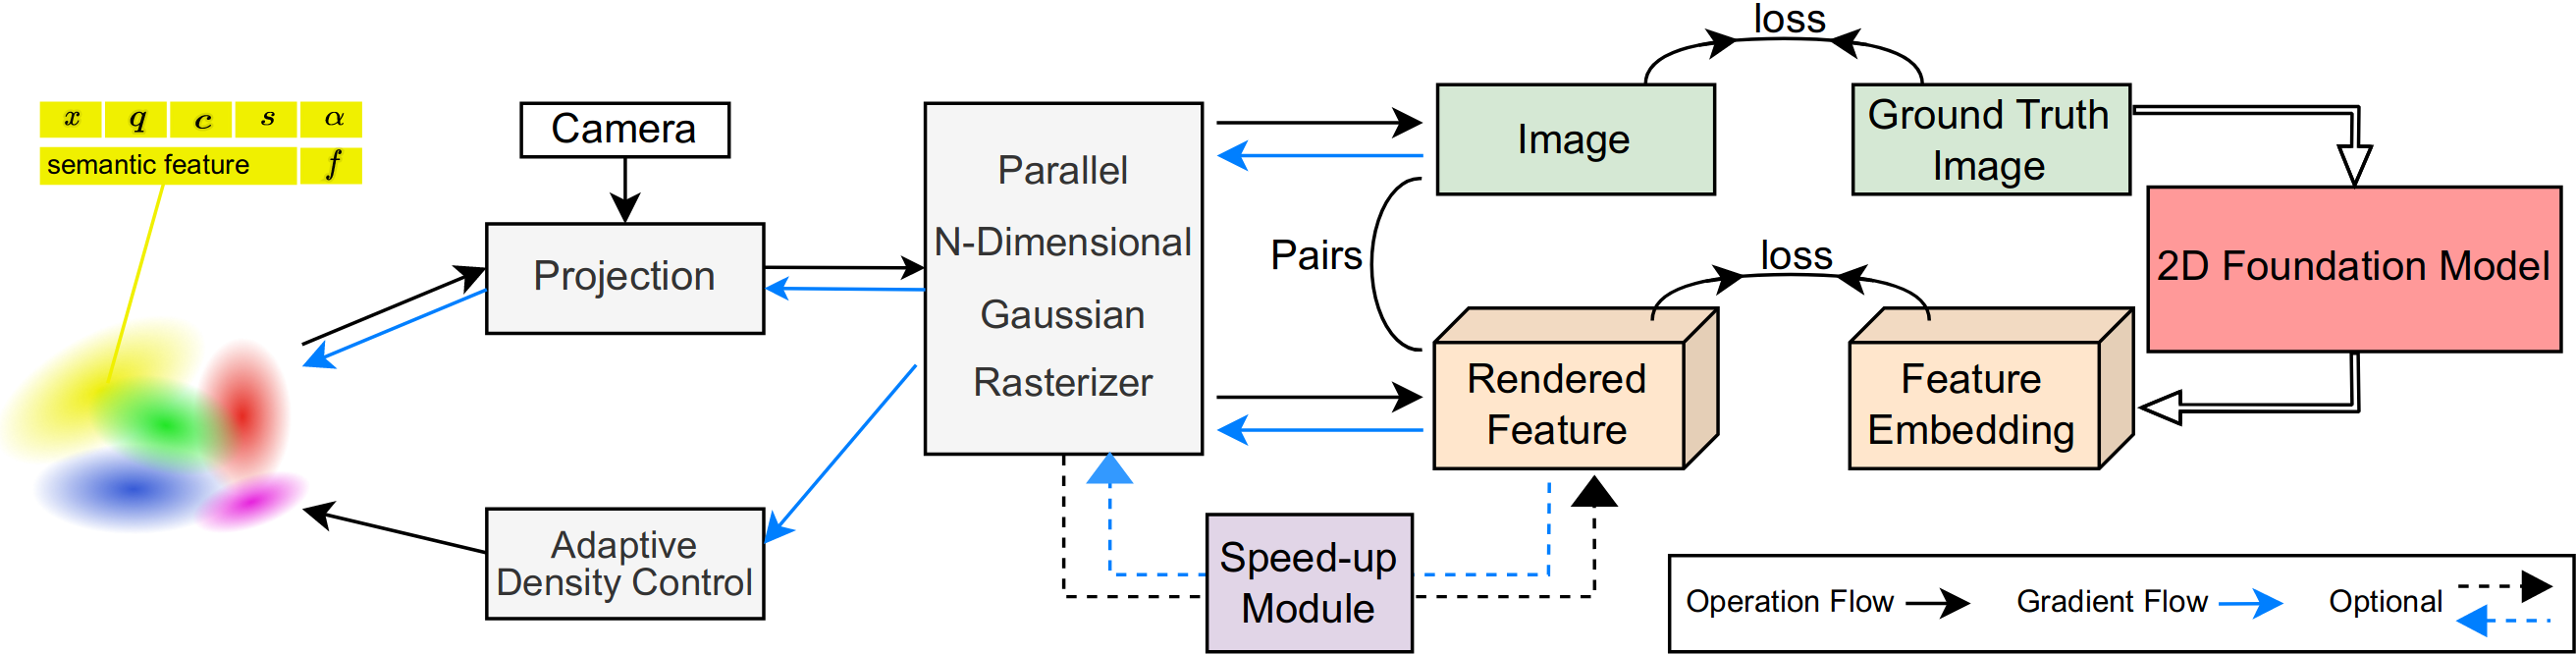
\includegraphics[width=4\linewidth]{feature-3dgs-overview.png}
			}
		\end{minipage}
		\hspace{\fill}
	}

	\begin{block}{Rasterization\hfill Semantic Rendering Pipeline \romannum{4}}
		\par \alert{Rasterization}: tiled and implemented in CUDA.
		\begin{itemize}[<+(1)->]
			\mode<presentation>{\setlength{\itemsep}{1.5ex}}
			\item \alert<.(1)|handout:0>{Divide} the screen space into tiles (CUDA thread blocks).
			\item \alert<.(1)|handout:0>{Group} the Gaussians by view frustum and tile index.
			\item \alert<.(1)|handout:0>{Sort} the Gaussians by front-to-back depth order.
			\item \alert<.(1)|handout:0>{Blend} each pixel within a tile in parallel (CUDA threads).
		\end{itemize}
	\end{block}
\end{frame}

\begin{frame}
	\mode<presentation>{\Frametitle{Semantic Rendering Pipeline \romannum{5}}}

	\mode<presentation>{\blfootnote{\href{http://arxiv.org/abs/2312.03203}{(CVPR Highlight, 2024) Feature 3DGS: Supercharging 3D Gaussian Splatting to Enable Distilled Feature Fields}}}
	\begin{block}{Inverse Rendering\hfill Semantic Rendering Pipeline \romannum{5}}
		\par \alert<1->{Inverse rendering}: guided by image-wise photometric loss.
		\footnote{\(\gamma=1, \lambda=0.2.\)}
		\mode<article>{(equation \ref{eq:feature-3dgs-loss}, \ref{eq:feature-3dgs-appearance-loss} and \ref{eq:feature-3dgs-semantic-loss})}
		\resetcolorseries[2]{marknode-color-series}
		\resetcolorseries[2]{annotation-color-series}
		\begin{equation}\label{eq:feature-3dgs-loss}
			\mathcal{L} = \mathcal{L}_{appearance} + \gamma \mathcal{L}_{semantics}
		\end{equation}
		\vspace*{1.2em}
		\begin{alignat}{2}
			\label{eq:feature-3dgs-appearance-loss} & \mathcal{L}_{appearance} &  & = (1-\lambda) \mathcal{L}_{1} \left(
			\tikzmarknode{n0}{\colorbox{marknode-color-series!![0]}{\(\mathbf{C}\)}}
			,
			\tikzmarknode{n1}{\colorbox{marknode-color-series!![0]}{\(\hat{\mathbf{C}}\)}}
			\right) + \lambda \mathcal{L}_{D-SSIM}\left(\mathbf{C}, \hat{\mathbf{C}}\right)                              \\
			\label{eq:feature-3dgs-semantic-loss}   & \mathcal{L}_{semantics}  &  & = \mathcal{L}_{1} \left(
			\tikzmarknode{n2}{\colorbox{marknode-color-series!![1]}{\(\mathbf{F}\)}}
			,\tikzmarknode{n3}{\colorbox{marknode-color-series!![1]}{\(\hat{\mathbf{F}}\)}}
			\right) = \sum_{h=1}^{H} \sum_{w=1}^{W} \Vert \mathbf{f}{(h, w)} - \hat{\mathbf{f}}{(h, w)} \Vert_1
		\end{alignat}
		\begin{annotatedEquationEnv}
			\annotatedEquation{color}{n0}{north}{0em}{1.2em}{south east}{annotation-color-series!!}{captured RGB image (ground-truth)}{west}
			\annotatedEquation{color}{n1}{north}{0em}{1em}{south west}{annotation-color-series!!}{rendered RGB image}{east}
			\textcolor{annotation-color-series!!+}{}%
			\annotatedEquation{color}{n2}{south}{0em}{-1.5em}{north east}{annotation-color-series!!}{inferred semantic feature map}{west}
			\annotatedEquation{color}{n3}{south}{0em}{-1.5em}{north west}{annotation-color-series!!}{rendered semantic feature map}{east}
		\end{annotatedEquationEnv}
		\vspace*{1.5em}
	\end{block}
\end{frame}

\begin{frame}
	\Frametitle{Speed-up Module}
	\begin{block}<+->{Motivation}
		\par Too \emph{inefficient} to embed naively,
		\begin{enumerate}[<+->]
			\mode<presentation>{\setlength{\itemsep}{1.5ex}}
			\item \alert<.>{High dimension:} latent features in large foundation models.
			      \footnote{e.g. \(512\) for CLIP; \(256\) for SAM.}
			\item \alert<.>{Large quantities:} millions of Gaussians in a scene.
		\end{enumerate}
	\end{block}
	\mode<presentation>{\vspace*{\fill}}
	\begin{block}<+->{Solution}
		\begin{enumerate}[<+->]
			\mode<presentation>{\setlength{\itemsep}{1.5ex}}
			\item \alert<.>{Compactness:} to embed Gaussians with more compact vectors, \(\dim = D^{\,\prime} < D\).
			\item \alert<.>{Alignment:} to align the dimensionalities using a lightweight decoder.\footnote{Lightweight decoder: In practice, a \(1\times 1\) convolutional layer or a fully-connected layer.}
		\end{enumerate}
	\end{block}
	\mode<presentation>{\blfootnote{\href{http://arxiv.org/abs/2312.03203}{(CVPR Highlight, 2024) Feature 3DGS: Supercharging 3D Gaussian Splatting to Enable Distilled Feature Fields}}}
\end{frame}

\begin{frame}
	\Frametitle{Summary}
	\mode<presentation>{\blfootnote{\href{http://arxiv.org/abs/2312.03203}{(CVPR Highlight, 2024) Feature 3DGS: Supercharging 3D Gaussian Splatting to Enable Distilled Feature Fields}}}
	\begin{block}{Limitations}
		\begin{enumerate}[<+->]
			\mode<presentation>{\setlength{\itemsep}{1.5ex}}
			\item Inefficiency
			      \mode<presentation>{\vspace*{1.5ex}}
			      \begin{itemize}
				      \mode<presentation>{\setlength{\itemsep}{1.5ex}}
				      \item ``Speed-up module'' is not enough,
				            \uncover<+->{
					            \mode<presentation>{\vspace*{1.5ex}}
					            \par \(\dim = 128\) embedding for millions of Gaussians.
				            }
			      \end{itemize}
			      \mode<presentation>{\vspace*{1.5ex}}
			\item 3D Inconsistency \& Inaccuracy
			      \mode<presentation>{\vspace*{1.5ex}}
			      \begin{itemize}
				      \mode<presentation>{\setlength{\itemsep}{1.5ex}}
				      \item 2D foundation models are still 2D.
			      \end{itemize}
		\end{enumerate}
	\end{block}
\end{frame}

